\documentclass[smaller]{beamer}

\usepackage[utf8]{inputenc}
\usepackage{polski}
\usepackage{listings}
\usepackage{syntax}


\definecolor{javared}{rgb}{0.6,0,0} % for strings
\definecolor{javagreen}{rgb}{0.25,0.5,0.35} % comments
\definecolor{javapurple}{rgb}{0.5,0,0.35} % keywords
\definecolor{javadocblue}{rgb}{0.25,0.35,0.75} % javadoc

 \lstloadlanguages{
         Java,XML
 }

 \lstset{language=XML,
  basicstyle=\ttfamily,
  columns=fullflexible,
  showstringspaces=false,
  escapechar={§},
  commentstyle=\color{gray}\upshape
}
 \lstset{language=Java,
%          basicstyle=\footnotesize\ttfamily, % Standardschrift
         basicstyle=\footnotesize\ttfamily, % Standardschrift
         %numbers=left,               % Ort der Zeilennummern
         numberstyle=\tiny\color{black},          % Stil der Zeilennummern
         stepnumber=1,               % Abstand zwischen den Zeilennummern
         numbersep=5pt,              % Abstand der Nummern zum Text
         tabsize=3,                  % Groesse von Tabs
% 	inputencoding=utf8, extendchars=\true
         extendedchars=true,         %
         breaklines=true,            % Zeilen werden Umgebrochen
keywordstyle=\color{javapurple}\bfseries,
stringstyle=\color{javared},
escapechar={§},
commentstyle=\color{javagreen},
morecomment=[s][\color{javadocblue}]{/**}{*/},
    		frame=b,         
 %        keywordstyle=[1]\textbf,    % Stil der Keywords
 %        keywordstyle=[2]\textbf,    %
 %        keywordstyle=[3]\textbf,    %
 %        keywordstyle=[4]\textbf,   \sqrt{\sqrt{}} %
         stringstyle=\color{blue}\ttfamily, % Farbe der String
         showspaces=false,           % Leerzeichen anzeigen ?
         showtabs=false,             % Tabs anzeigen ?
         xleftmargin=10pt,
         framexleftmargin=10pt,
         framexrightmargin=5pt,
         framexbottommargin=4pt,
         %backgroundcolor=\color{lightgray},
         showstringspaces=false      % Leerzeichen in Strings anzeigen ?        
 }
    %\DeclareCaptionFont{blue}{\color{blue}} 
  %\captionsetup[lstlisting]{singlelinecheck=false, labelfont={blue}, textfont={blue}}
  \usepackage{caption}
\DeclareCaptionFont{white}{\color{white}}
\DeclareCaptionFormat{listing}{\colorbox[cmyk]{0.43, 0.35, 0.35,0.01}{\parbox{\textwidth}{\hspace{15pt}#1#2#3}}}
\captionsetup[lstlisting]{format=listing,labelfont=white,textfont=white, singlelinecheck=false, margin=0pt, font={bf,footnotesize}}



\usepackage{tikz}
    \usetikzlibrary{fit,calc,decorations.pathreplacing,arrows,mindmap,shapes}
    \newcommand{\tikzref}[1]{% to define an anchor
        \tikz[remember picture]{%
            \coordinate (#1) at (0,0.5ex);%
        }%
    }
    \tikzstyle{transp}=[fill opacity=0.75,fill=white, inner sep=1.5mm]
    \tikzstyle{reverseclip}=[insert path={(current page.north east) --
        (current page.south east) --
        (current page.south west) --
        (current page.north west) --
        (current page.north east)}
    ]

\tikzset{every concept/.style={rectangle,minimum size=2cm, text width=2cm}}
\tikzset{level 1 concept/.append style={font=\sf, sibling angle=90,level distance = 27mm}}
\tikzset{level 2 concept/.append style={font=\sf, sibling angle=45,level distance = 17mm}}
\tikzset{onslide/.code args={<#1>#2}{%
  \only<#1>{\pgfkeysalso{#2}} 
}}
\tikzset{every node/.append style={scale=0.6}}  
\tikzset{%
	>=latex,  
	inject line/.style={%
        		color=red,line width=1pt,->
    	}
}

\usepackage{amsmath}
\usepackage{xspace}
\newcommand{\A}{\ensuremath{\mathcal{A}}\xspace}
\newcommand{\B}{\ensuremath{\mathcal{B}}\xspace}
\newcommand\pa[1]{\ensuremath{\left(#1\right)}}


\usetheme{Warsaw}
\title{Testowanie poprzez moduły Guice}
\author{Paweł Cesar Sanjuan Szklarz}
\date{9/04/2013}

\begin{document}

\frame{\titlepage}


\defverbatim[colored]\xmlInjection{%
\begin{lstlisting}[tabsize=2,frame=single,language=XML]
<bean id="exampleBean" class="examples.ExampleBean">
  <property name="beanOne"><ref bean="anotherExa§\tikzref{z1}§mpleBean"/></property>
  <property name="beanTwo" ref="§\tikzref{z2}§yetAnotherBean"/>
  <property name="integerProperty" value="1"/>
</bean>

<bean id="anotherExampleBean§\tikzref{b1}§" class="examples.AnotherBean"/>
<bean id="yetAnotherBean§\tikzref{b2}§" class="examples.YetAnotherBean">
  <property name="beanThree" ref="nested§\tikzref{z3}§Bean"/>
</bean>

<bean id="nestedBean§\tikzref{b3}§" class="examples.YetOther"/>
\end{lstlisting}}

\begin{frame}{Injektowanie zależności nie jest prostym mapowaniem}

\begin{alert}{Mit:}
Injektowanie zależności to prosta mapa \lstinline|Map<Type,Object>|
\end{alert}

\pause

\xmlInjection
\pause

\begin{tikzpicture}[overlay, remember picture]
	\path[inject line] (b1) edge [bend right] (z1);
	\path[inject line] (b2) edge [bend left] (z2);
	\path[inject line] (b3) edge [bend right] (z3);
\end{tikzpicture}

Konfiguracja Spring sprowadza się do \lstinline|Map<String,Bean>|??
\pause
\center
\alert{Nie, ale mało kto wie i używa pełną strukturę.}

\end{frame}


\defverbatim[colored]\guicePrivateModuleExamples{%
\begin{lstlisting}[tabsize=2,frame=single]
import com.google.inject.PrivateModule;
public class SimpleConfiguration extends PrivateModule {
    @Override
    protected void configure() {
        expose(ClientApi.class);
        bind(ClientApi.class).to(ClientApiImplementation.class);
        bind(ClientInternalApi.class).to(ClientInternal.class);
    }
}
\end{lstlisting}}


\defverbatim[colored]\guicePrivateModuleWithLibraries{%
\begin{lstlisting}[tabsize=2,frame=single]
public class ComplexConfiguration extends PrivateModule {
    @Override
    protected void configure() {
        expose(ClientApi.class);
        bind(ClientApi.class).to(ClientApiImplementation.class);
        bind(ClientInternalApi.class).to(ClientInternal.class);
        // more bindings
        install(new NestedModuleOne());
        install(new NestedModuleTwo());
    }
}
\end{lstlisting}}
\defverbatim[colored]\guicePrivateModuleWithLibrariesONE{%
\begin{lstlisting}[tabsize=2,frame=single]
public class NestedModuleOne extends PrivateModule {
    @Override
    protected void configure() {
        expose(LibraryOneApi.class);
        bind(LibraryOneApi.class).to(LibraryOneInternal.class);
        bind(CommonLogApi.class).toInstance(new CommonLogApi() {
            @Override
            public void log(String message) {
                System.out.println("Library ONE log:" + message);
            }
        });
    }
}
\end{lstlisting}}
\defverbatim[colored]\guicePrivateModuleWithLibrariesTWO{%
\begin{lstlisting}[tabsize=2,frame=single]
public class NestedModuleTwo extends PrivateModule {
    @Override
    protected void configure() {
        expose(LibraryTwoApi.class);
        bind(LibraryTwoApi.class).to(LibraryTwoInternal.class);
        bind(CommonLogApi.class).toInstance(new CommonLogApi() {
            @Override
            public void log(String message) {
                System.out.println("Library TWO log:" + message);
            }
        });
    }
}
\end{lstlisting}}

\defverbatim[colored]\guiceFinalMockingModulesTest{%
\begin{lstlisting}[tabsize=2,frame=single]
@Guice(modules = {SimpleConfiguration.class,SimpleConfigurationTestIzolated.LibsMockTestModule.class})
public class SimpleConfigurationTestIzolated {
    public static class LibsMockTestModule extends AbstractModule {
        static LibraryTwoApi twoApi = mock(LibraryTwoApi.class);
        static LibraryOneApi oneApi = mock(LibraryOneApi.class);
        @Override
        protected void configure() {
            bind(LibraryOneApi.class).toInstance(oneApi);
            bind(LibraryTwoApi.class).toInstance(twoApi);
        }
    }
    @Inject
    private ClientApi clientApi;
    @Test
    public void testMockingInjection(){
        clientApi.testLogging();
        verify(LibsMockTestModule.oneApi).oneApiCall();
        verify(LibsMockTestModule.twoApi).twoApiCall();
    }
}
\end{lstlisting}}


\defverbatim[colored]\guicePrivateModuleExamplesTest{%
\begin{lstlisting}[tabsize=2,frame=single]
    @Inject
    private Injector injector;
    @Test
    public void testExposedKeys(){
        assertNotNull(injector.getExistingBinding(Key.get(ClientApi.class)));
        assertNull(injector.getExistingBinding(Key.get(ClientInternalApi.class)));
    }
\end{lstlisting}}
\begin{frame}{Pełna struktura - na przypadek Guice}

W Guice można zrobić \lstinline|PrivateModule| i dać dostęp do ograniczonej listy kluczy \lstinline|Key<?>|:

\guicePrivateModuleExamples
\pause
\guicePrivateModuleExamplesTest
\end{frame}


\begin{frame}{Pełna struktura - na przypadek Guice}

Otrzymujemy injektor który "chowa" wewnętrzne klucze.

\center
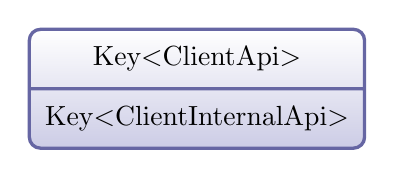
\begin{tikzpicture}[
    grow=down,
    level 1/.style={sibling distance=5.5cm,level distance=3.2cm},
    level 2/.style={sibling distance=5.5cm, level distance=1.7cm},
    edge from parent/.style={very thick,draw=blue!40!black!60,
        shorten >=5pt, shorten <=5pt},
    edge from parent path={(\tikzparentnode.south) -- (\tikzchildnode.north)},
    kant/.style={text width=2cm, text centered, sloped},
    every node/.style={text ragged, inner sep=2mm},
    punkt/.style={rectangle, rounded corners, shade, top color=white,
    bottom color=blue!50!black!20, draw=blue!40!black!60, very
    thick }
    ]

\node[punkt, rectangle split, rectangle split,
            rectangle split parts=2] {
		\lstinline|Key<ClientApi>|
		\nodepart{second}
		\lstinline|Key<ClientInternalApi>|
            };
\end{tikzpicture}

\guicePrivateModuleExamples

\end{frame}

\begin{frame}{Wynik: Drzewo injektorów}
\guicePrivateModuleWithLibraries
\end{frame}
\begin{frame}{Wynik: Drzewo injektorów}
\guicePrivateModuleWithLibrariesONE
\end{frame}
\begin{frame}{Wynik: Drzewo injektorów}
\guicePrivateModuleWithLibrariesTWO
\end{frame}

\begin{frame}{Wynik: Drzewo injektorów}
\center
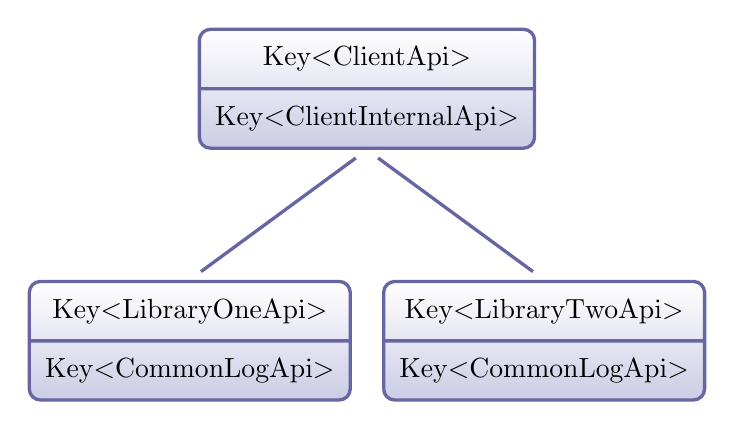
\begin{tikzpicture}[
    grow=down,
    level 1/.style={sibling distance=4.5cm,level distance=3.2cm},
    level 2/.style={sibling distance=5.5cm, level distance=1cm},
    edge from parent/.style={very thick,draw=blue!40!black!60,
        shorten >=5pt, shorten <=5pt},
    edge from parent path={(\tikzparentnode.south) -- (\tikzchildnode.north)},
    kant/.style={text width=2cm, text centered, sloped},
    every node/.style={text ragged, inner sep=2mm},
    punkt/.style={rectangle, rounded corners, shade, top color=white,
    bottom color=blue!50!black!20, draw=blue!40!black!60, very
    thick }
    ]

\node[punkt, rectangle split, rectangle split,
            rectangle split parts=2] {
		\lstinline|Key<ClientApi>|
		\nodepart{second}
		\lstinline|Key<ClientInternalApi>|
            }
        %child 1
        child {
            node [punkt,rectangle split, rectangle split,
            rectangle split parts=2] {
		\lstinline|Key<LibraryOneApi>|
                \nodepart{second}
		\lstinline|Key<CommonLogApi>|
            }
        }
        %child 2
        child {
            node [punkt, rectangle split, rectangle split parts=2]{
		\lstinline|Key<LibraryTwoApi>|
                \nodepart{second}
		\lstinline|Key<CommonLogApi>|
            }
          };
\end{tikzpicture}
\end{frame}

\begin{frame}{Jak testować lepiej?}
\begin{itemize}
\item<1-> Aplikacja jako drzewo injektorów
\item<2-> Izolacja komponentów w hierarchii
\item<3-> Tworzenie testowych modułów
\end{itemize}

\center
\begin{tikzpicture}[
    grow=down,
    level 1/.style={sibling distance=2cm,level distance=1.5cm},
    level 2/.style={sibling distance=1cm, level distance=1.5cm},
    level 3/.style={sibling distance=1cm, level distance=1cm},
    edge from parent/.style={very thick,draw=blue!40!black!60, shorten >=5pt, shorten <=5pt},
    edge from parent path={(\tikzparentnode.south) -- (\tikzchildnode.north)},
    kant/.style={text width=1cm, text centered, sloped},
    punkt/.style={rectangle, rounded corners, shade, top color=white,bottom color=blue!50!black!20, draw=blue!40!black!60, very thick },
    isolate/.style={rectangle, rounded corners, shade, top color=white,bottom color=blue!50!black!20, draw=red, very thick },
    testmodule/.style={draw=orange},
    deletedmodule/.style={opacity=0.3}
    ]

\node[punkt,onslide=<2->{isolate}, rectangle split,rectangle split parts=2] {
		Keys
                \nodepart{second}
		Keys
            }
        %child 1
        child {
            node [punkt,onslide=<3->{testmodule},rectangle split, rectangle split,
            rectangle split parts=2] {
		{\color<2->{red}Keys}
                \nodepart{second}
                  {\onslide<1-2>{Keys}}
            }
        child {
            node [punkt,onslide=<3->{deletedmodule}, rectangle split, rectangle split,
            rectangle split parts=2] {
		Keys
                \nodepart{second}
		Keys
            }
        }
        child {
            node [punkt,onslide=<3->{deletedmodule}, rectangle split, rectangle split,
            rectangle split parts=2] {
		Keys
                \nodepart{second}
		Keys
            }
        }
        child {
            node [punkt,onslide=<3->{deletedmodule}, rectangle split, rectangle split,
            rectangle split parts=2] {
		Keys
                \nodepart{second}
		Keys
            }
        }
        }
        %child 2
        child {
            node [punkt,onslide=<3->{testmodule}, rectangle split, rectangle split parts=2]{
		{\color<2->{red}Keys}
                \nodepart{second}
                  {\onslide<1-2>{Keys}}
            }
        child {
            node [punkt,onslide=<3->{deletedmodule}, rectangle split, rectangle split,
            rectangle split parts=2] {
		Keys
                \nodepart{second}
		Keys
            }
        }
          };
\end{tikzpicture}

\end{frame}

\begin{frame}{Przyklad mockowania modułów}
\guiceFinalMockingModulesTest
\end{frame}

\begin{frame}{Testy integracyjne}
\center
A co jak injektor będzie rozproszony po wielu komputerach??

\center
\alert{DEMO}

\end{frame}

\end{document}
